\documentclass[tikz,border=7pt]{standalone}

\usepackage[T1]{fontenc}
\usepackage{amsmath}
\usepackage{newtxtext,newtxmath}
\usetikzlibrary{arrows.meta,backgrounds,calc,decorations.pathreplacing,positioning}

\definecolor{extendedcolor}{HTML}{EE3377}
\definecolor{pointcolor}{HTML}{009988}
\definecolor{ink}{HTML}{263238}
\definecolor{muted}{HTML}{60717A}
\definecolor{paper}{HTML}{F7F8F8}
\definecolor{linegray}{HTML}{455A64}

\tikzset{
  box/.style={
    draw=ink,
    fill=white,
    text=ink,
    line width=0.75pt,
    rounded corners=3pt,
    minimum height=1.15cm,
    align=center,
    inner xsep=5pt,
    inner ysep=5pt,
    font=\small
  },
  catalogue/.style={
    box,
    fill=paper,
    draw=ink,
    line width=1.0pt,
    minimum width=3.55cm,
    text width=3.25cm
  },
  rowbox/.style={
    box,
    minimum width=2.70cm,
    minimum height=1.45cm,
    text width=2.40cm,
    font=\small
  },
  rowgreen/.style={rowbox,fill=paper,draw=muted},
  rowpink/.style={rowbox,fill=extendedcolor!9,draw=extendedcolor!80!black},
  lowerbox/.style={
    box,
    minimum width=2.70cm,
    minimum height=1.45cm,
    text width=2.40cm,
    font=\small
  },
  extended/.style={box,fill=extendedcolor!9,draw=extendedcolor!80!black,minimum width=2.55cm,text width=2.25cm},
  pointlike/.style={lowerbox,fill=pointcolor!14,draw=pointcolor!85!black},
  lowerpink/.style={lowerbox,fill=extendedcolor!10,draw=extendedcolor!80!black},
  final/.style={lowerbox,fill=ink,draw=ink,text=white,line width=1.0pt},
  outputmap/.style={lowerbox,fill=extendedcolor!10,draw=extendedcolor!80!black},
  smooth/.style={
    box,
    fill=paper,
    text=ink,
    draw=muted,
    line width=0.85pt,
    minimum width=3.15cm,
    text width=2.85cm,
    font=\small
  },
  comparison/.style={
    box,
    fill=extendedcolor!10,
    draw=extendedcolor!80!black,
    minimum width=5.25cm,
    text width=4.95cm
  },
  iolabel/.style={
    text=muted,
    font=\sffamily\bfseries\scriptsize,
    inner sep=0pt
  },
  iobrace/.style={
    decorate,
    decoration={brace,amplitude=3.5pt},
    draw=muted,
    line width=0.65pt
  },
  flow/.style={
    -{Latex[length=2.2mm,width=1.6mm]},
    draw=linegray,
    line width=0.78pt,
    rounded corners=1.5pt,
    line cap=round,
    line join=round
  },
  auxflow/.style={
    flow,
    dash pattern=on 3pt off 2pt
  },
  mergepath/.style={
    draw=linegray,
    line width=0.78pt,
    line cap=round,
    line join=round
  }
}

\begin{document}
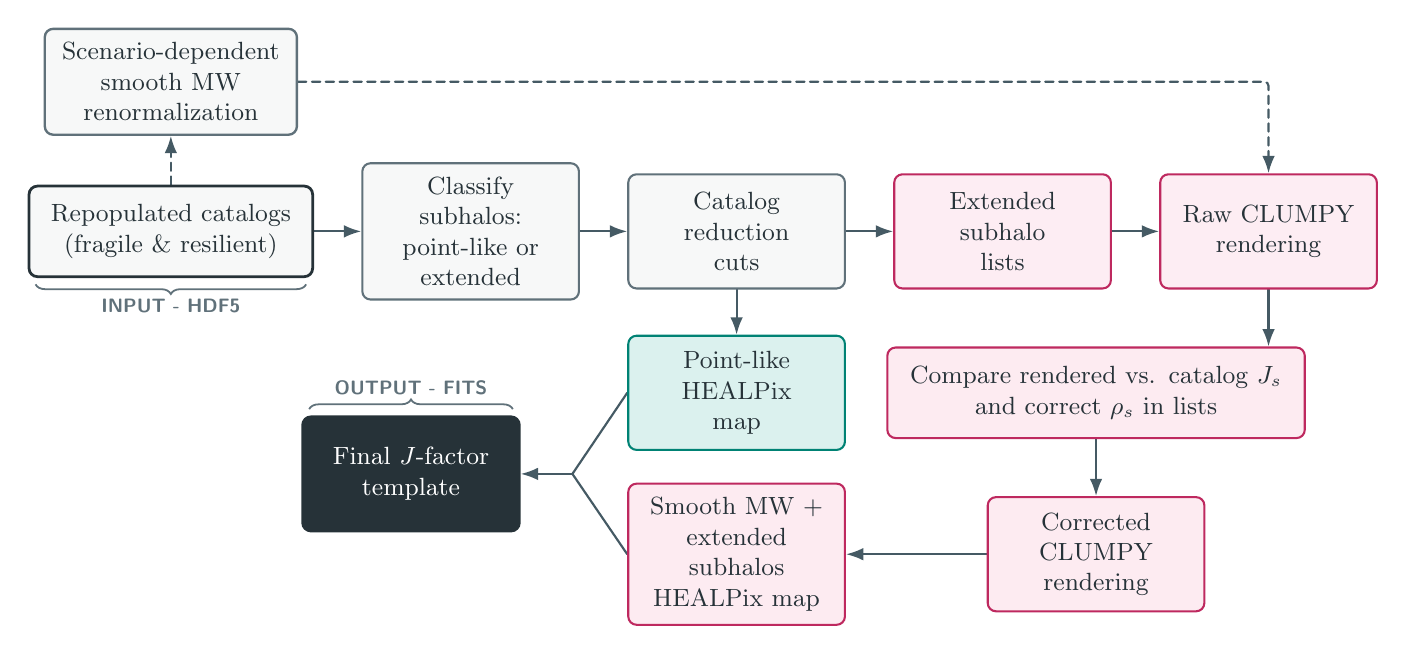
\begin{tikzpicture}

  % Main horizontal catalogue-to-CLUMPY sequence.
  \node[smooth] (renorm) at (0,1.90)
    {Scenario-dependent\\smooth MW\\renormalization};

  \node[catalogue] (catalogues) at (0,0)
    {Repopulated catalogs\\(fragile \& resilient)};

  \node[rowgreen,right=0.60cm of catalogues] (classify)
    {Classify subhalos:\\point-like or\\extended};

  \node[rowgreen,right=0.60cm of classify] (cuts)
    {Catalog reduction\\cuts};

  \node[rowpink,right=0.60cm of cuts] (lists)
    {Extended subhalo\\lists};

  \node[rowpink,right=0.60cm of lists] (raw)
    {Raw CLUMPY\\rendering};

  % Lower point-like and corrected-CLUMPY branches.
  \node[pointlike] (pointmap) at ($(cuts.center)+(0,-2.05)$)
    {Point-like HEALPix\\map};

  \node[comparison] (compare) at (11.75,-2.05)
    {Compare rendered vs. catalog \(J_s\)\\and correct \(\rho_s\) in lists};

  \node[lowerpink] (corrected) at (11.75,-4.10)
    {Corrected CLUMPY\\rendering};

  \node[outputmap] (smoothmap) at ($(cuts.center)+(0,-4.10)$)
    {Smooth MW +\\extended subhalos\\HEALPix map};

  \node[final] (finalmap) at (3.05,-3.08)
    {Final \(J\)-factor\\template};

  \draw[iobrace,decoration={brace,mirror,amplitude=3.5pt}]
    ([xshift=0.10cm,yshift=-0.08cm]catalogues.south west) --
    ([xshift=-0.10cm,yshift=-0.08cm]catalogues.south east)
    node[midway,below=5pt,iolabel] {INPUT - HDF5};

  \draw[iobrace]
    ([xshift=0.10cm,yshift=0.08cm]finalmap.north west) --
    ([xshift=-0.10cm,yshift=0.08cm]finalmap.north east)
    node[midway,above=5pt,iolabel] {OUTPUT - FITS};

  \coordinate (merge) at (5.10,-3.08);

  % Arrows are drawn behind the nodes so no connector crosses text.
  \begin{scope}[on background layer]
    \draw[flow] (catalogues.east) -- (classify.west);
    \draw[flow] (classify.east) -- (cuts.west);
    \draw[flow] (cuts.east) -- (lists.west);
    \draw[flow] (lists.east) -- (raw.west);

    \draw[auxflow] (catalogues.north) -- (renorm.south);
    \draw[auxflow] (renorm.east) -- ++(0.55,0) -| (raw.north);

    \draw[flow] (cuts.south) -- (pointmap.north);

    \draw[flow] (raw.south) -- (raw.south |- compare.north);
    \draw[flow] (compare.south) -- (corrected.north);
    \draw[flow] (corrected.west) -- (smoothmap.east);

    \draw[mergepath] (pointmap.west) -- (merge);
    \draw[mergepath] (smoothmap.west) -- (merge);
    \draw[flow] (merge) -- (finalmap.east);
  \end{scope}

\end{tikzpicture}
\end{document}
